\documentclass[twoside]{article}
%-------------------------------------------------------------------------------------------------%
\usepackage[utf8]{inputenc}
\usepackage[english]{babel}
\usepackage{biblatex}
\usepackage[a4paper, total={6in, 9.5in}]{geometry}
\usepackage[T1]{fontenc}
\usepackage[nottoc,numbib]{tocbibind}
\usepackage{multicol}
\usepackage{tabularx}
\usepackage{graphicx}
\usepackage{titling}
\usepackage{tocloft}
\usepackage[labelfont=bf]{caption}
\captionsetup{belowskip=15pt, aboveskip=0pt}
\usepackage{subcaption}
\usepackage{hologo}
\usepackage[hidelinks]{hyperref}
\usepackage{csquotes}
\usepackage{amsmath}
\usepackage{amssymb}
\usepackage{minted}
\usepackage{multicol}
\usepackage{listings}
\newenvironment{longlisting}{\captionsetup{type=listing}}{}
\usemintedstyle{emacs}
\setminted{
    breaklines,
    autogobble,
}

%-------------------------------------------------------------------------------------------------%
\graphicspath{ {./images/} }
\addbibresource{format.bib}
%-------------------------------------------------------------------------------------------------%
\renewcommand\cftsecpagefont{\normalfont}
\renewcommand{\cftsecleader}{\cftdotfill{\cftsecdotsep}}
\renewcommand\cftsecdotsep{\cftdot}
\renewcommand\cftsubsecdotsep{\cftdot}
\pretitle{
  \begin{center}
    \Huge\bfseries }
\renewcommand\maketitlehookb{
  \begin{center}
    \Large {An Investigatory Project Report}\\[0.25in] 
\includegraphics[scale =
      0.75]{tos_logo.jpeg}\\[0.25in] \bfseries {Submitted by}
  \end{center}
}
\predate{}
\postdate{}
\renewcommand\maketitlehookd{
  \begin{center}
    \large{ The Orchid School\\ Baner Pune 411045\\[0.3cm] \textbf{2020-2021}\\ }
  \end{center}
}
%-------------------------------------------------------------------------------------------------%
\title{RSA Encryption Tool}
\author{ Nebhrajani, Aditya V.}%\\ Magapu,Abhimanyu\\ Sharma, Galav\\ }
\date{}
%-------------------------------------------------------------------------------------------------%

\begin{document}

\maketitle
\thispagestyle{empty}

\cleardoublepage


{\center
\includegraphics[scale = 0.5]{tos_logo.jpeg}\\[0.25in]} {\center\LARGE The Orchid School\\}
{\center\huge\textbf {Certificate}\\[0.5cm]}

This is to certify that Aditya V. Nebhrajani of Class XII I1 has successfully completed the Informatics Practices
Investigatory Project in the partial fulfillment of curriculum of Central Board of Secondary
Education (CBSE) leading to award of Annual Examination of the year 2020-2021.\\[1cm]


\begin{center}
\begin{tabularx}{\textwidth}{>{\centering\arraybackslash}X  >{\centering\arraybackslash}X}
External Examiner & Teacher In-Charge \\ & (Jayashree Samudra)\\[1.5cm] Unit Head & Principal \\ (Netre
Kulkarni) & (Namrata Majhail) \\
\end{tabularx}
\end{center}


\cleardoublepage
\section*{Acknowledgements}
\addcontentsline{toc}{section}{Acknowledgements}

No project can ever be completed without the graceful contribution of many, many people.\\

I would, first and foremost, like to express my gratitude to our IP teacher, Ms. Jayashree Samudra
for her valuable advice and inputs which enhanced the quality of my work. This project could not
have been completed successfully without her help. I would also like to thank Netre Di for her
encouragement and support, and our respected principal Namrata Di for giving me an opportunity to
work on such an intriguing topic. \\

This entire project was written on open source software, using open source programming and markup
languages. I am hence deeply indebted to the open source community at large. I would like to
separately acknowledge the GNU Emacs\footnote{The Emacs text editor/eLISP REPL:
https://www.gnu.org/software/emacs/}, \LaTeX\footnote{\LaTeX\ document creation system:
https://www.latex-project.org/}, Python\footnote{Python programming language:
https://www.python.org/} and the StackExchange\footnote{StackExchange forums:
https://stackexchange.com/} communities for their powerful -- and open source -- tools.\\

Lastly, I would like to thank my parents for their love and guidance without which nothing can be
accomplished.

\cleardoublepage
\tableofcontents

\cleardoublepage
\listoffigures

\cleardoublepage
\renewcommand\listoflistingscaption{Source Code Listings}
\listoflistings
\addcontentsline{toc}{section}{Source Code Listings}
\cleardoublepage

\section{Introduction}
Democratic governments the world over have a similar system of guaranteeing rights to people.
However, one right which is still not guaranteed by most is the right to privacy. Prior to the
advent of computer technology, privacy was easy to ensure: one had but to close the door or seal a letter.
Things have changed since then: humans communicate more and more over the Internet. This makes our
communications less private, since the medium of communication is not secure.

In any case, there are tremendous vested interests in invading people's privacy, from showing more
personalised ads to societal control and conditioning. After whistleblower Edward Snowden leaked
the United States' National Security Agency's highly classified information, it is public domain
knowledge that not only companies but also governments invade our privacy to their own ends.

It is difficult to overstate how morally incorrect and dangerous such a practice is. Snowden put the
situation excellently:

\begin{displayquote}
  ``Arguing that you don't care about privacy because you have nothing to hide is no different than
  saying you don't care about free speech because you have nothing to say.''
\end{displayquote}

The irony of the situation is that most people are aware that companies such as Google, Microsoft and Facebook
steal their data\footnote{Reference: Ask anyone.}, but they do nothing about it. This is best
explained through consumers preferring convenience over privacy. Google is easier to use than
DuckDuckGo, and is better developed. To expect anybody other than a few highly privacy-conscious
individuals to stop using Instagram and Windows 10 is not an ideal solution. Instead, the convenience
of encryption needs to be available to the general public in a user-friendly interface. Ideas like
PGP have tried and fallen into obscurity, PAKE didn't gain traction\cite{pake}, and people are
trusting, or trying to trust, WhatsApp's `end-to-end-encryption'. There is an opening for a system
that lets people secure their privacy while also being accessible and easy to
use.\cite{hackernews}\cite{gtank}

This project is an attempt to remedy this situation by building a framework for quick and easy to
use encryption. It's written in Python, which makes it easy to port or include in other
applications. The interactive CLI and Pandas database are merely for demonstration purposes.
Ideally, this project should be used as a module or as part of a larger communication application.


\cleardoublepage

\section{Cryptography}

\subsection{In History}
Since time immemorial, kings, queens, and armies have relied on the privacy of their communications
to communicate battle plans to units spread over a large area. Other people reliant on privacy were
secret lovers, those inciting rebellion, and even Mary Queen of Scots.

Privacy was ensured by somehow obscuring the original message using methods such as steganography or
cryptography. Steganography is of less interest to us, as it involves physically hiding a message,
for instance, by engraving it in a hidden place. The other method, cryptography, involved taking the
original message, the `plaintext', and converting it via an algorithm to an obscure mess of letters,
the `ciphertext'. The receiver then performed the reverse algorithm and retrieved the plaintext.
Thus, even if the message were intercepted, it could not be read and its information exploited.\footnote{Image
credit: The Code Book: The Science of Secrecy from Ancient Egypt to Quantum Cryptography, Simon
Singh. OCLC: 59459928}

\begin{figure}[H]
  \centering
  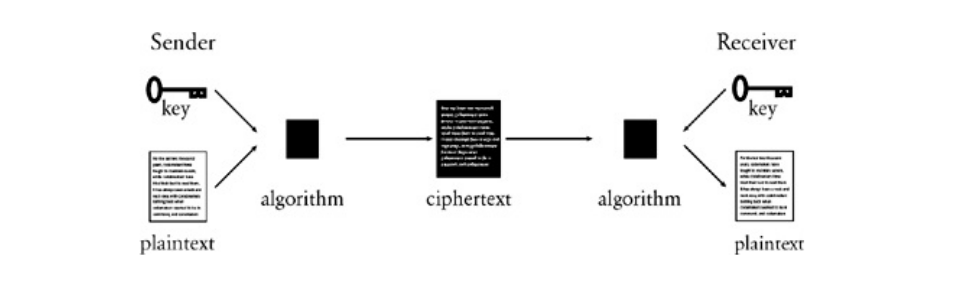
\includegraphics[scale=0.3]{cryp.png}
  \caption{Principle of encryption}
\end{figure}

In cryptography, the security of the whole system depends not on the security of the communication
medium but rather on the algorithm used. An example is the very simple Caesar cipher\cite{caesar}:

\begin{displayquote}
  The action of a Caesar cipher is to replace each plaintext letter with a different one a fixed
number of places down the alphabet. The cipher illustrated here uses a left shift of three, so that
(for example) each occurrence of E in the plaintext becomes B in the ciphertext.
\end{displayquote}


In this case, the `key' would be the number of places to shift each letter by, or the `shift'. The
Caesar cipher, like many others of its time, was broken by frequency analysis: given a long enough
sample of the ciphertext, a cryptanalyst could replace the most frequently occurring letter by the
one used most in the English alphabet (`e'), or the second most used (`t'), and so on. By trial and
error, the original message is soon revealed. In fact, the cipher of Mary Queen of Scots was broken
by frequency analysis by a cryptanalyst called Thomas Phelippes. Once the cipher was broken, the
Babington plot was revealed, and she was executed, with the cracked cipher being the central
evidence in the case against Mary Queen of Scots.

Much later, during the Second World War, the Polish and British forces joined hands to crack the
German Enigma cipher, which used an Enigma machine to encrypt the plaintext. The Polish designed
machines to crack the Enigma code (called `bombes' for the loud noises they made), which were further refined
by Alan Turing, who insisted on spending time designing mechanical machines that could break the
cipher rather than spend time cracking the ciphers by hand. This was one of the first instances of
machines being used to encrypt plaintext, and with Turing, machines being used to break ciphers.


\subsection{Modern Methods and Some Mathematics}
The primary problems in cryptography are key distribution and the security of the ciphertext. While
the security of the ciphertext can, in theory, be ensured by using complicated algorithms
implemented by machines, the problem of secure key distribution remains. If the keys are distributed
through an insecure communication medium, this renders the algorithm a mere computational hurdle at
best.

\subsubsection{Diffie-Hellman Key Exchange}
To solve the problem of secure key-distribution, Diffie, Hellman, and Merkle created a method for
generating keys even on an insecure communication medium. \cite{diffie} The method is shown in
the figure below.\footnote{Image credit: Diffie-Hellman key exchange - Wikipedia/Wikimedia Commons}

\begin{figure}[H]
  \centering
  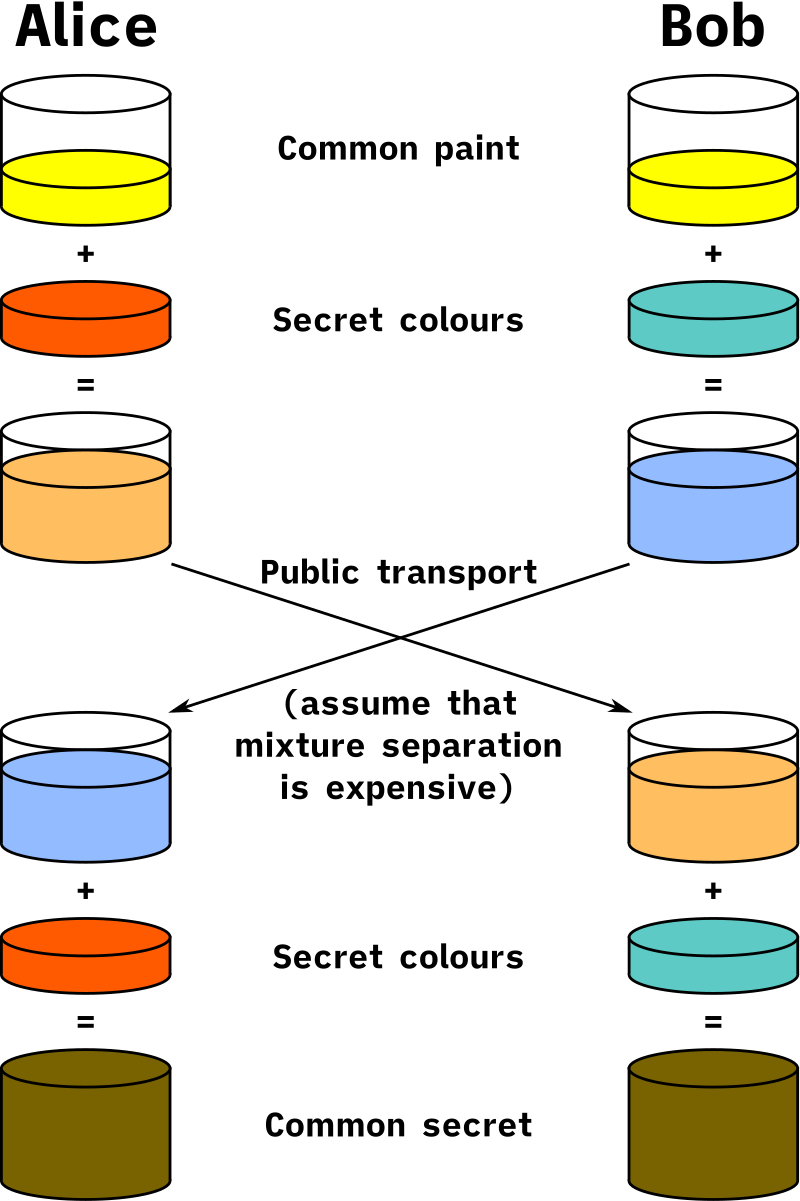
\includegraphics[scale=0.15]{diffie.png}
  \caption{Diffie-Hellman key exchange}
\end{figure}

As evident from the figure, a man-in-the-middle, despite having knowledge of the starting color
Alice and Bob agree on (yellow), and the intermediaries that they exchange (orange-tan and light
blue), he cannot find the final key since Alice and Bob do not exchange information about the secret
colors they use (blue and orange). In practice, of course, Alice and Bob use large numbers and the
modulo function (modulus from clock math) to eventually get the same secret key, which is a large
integer. This algorithm, proposed in 1976, is used to generate secret keys throughout the
Internet.  A simple generalisation of the principle used (using finite cyclic groups) is as follows
(a cyclic group is generated by a single element, and any element in the group can be obtained
by repeated group operations. A clock with an arithmetic of addition defined is a cyclic group of
order 12.):

\begin{enumerate}
\item Alice and Bob agree on a finite cyclic group $G$ (multiplicative) of order $n$ and a generating element $g$ in $G$. ($g$ is assumed to be known by all attackers.)
\item Alice picks a random natural number $a$ ($1 < a < n$) and sends $g^a$ to Bob.
\item Bob picks a random natural number $b$ ($1 < b < n$) and sends $g^b$ to Alice.
\item Alice finds $(g^b)^a$.
\item Bob finds $(g^a)^b$.
\item Since $(g^b)^a = (g^a)^b = g^{ab}$, both Alice and Bob have the same group element, which
  serves as the secret key.
\end{enumerate}


We note, however, that it is likely organisations with large budgets can crack Diffie-Hellman,
especially ones that use keys of 1024-bit lengths or less. Moreover, other vulnerabilities have been found in
Diffie-Hellman, as described in the paper \emph{Imperfect Forward Secrecy:
How Diffie-Hellman Fails in Practice}. \cite{imperfect} According to Adrian et al. around two-thirds
of popular HTTPS sites allow TLS using Diffie-Hellman and 1024-bit-keys. Some even allow legacy
512-bit keys. Two-thirds of the HTTPS servers analyzed also use common groups for generation,
meaning some primes are more `popular' than others. These vulnerabilities were exploited by the
paper and the Logjam attack was used to cryptanalyze Diffie-Hellman.

Diffie-Hellman inspired a much more powerful algorithm, the RSA asymmetric key encryption.

\subsubsection{RSA Encryption}
\label{section:rsamath}
RSA encryption\cite{rivest1978method}, named after Ron \textbf{R}ivest, Adi \textbf{S}hamir, and
Leonard \textbf{A}dleman, uses the concept of each user having two keys: one public key and one
private key. Assume these keys are pre-generated. Say Bob wants to send a message $M$ to Alice.
Alice's public key is a tuple of integers $(n, e)$ and her private key is an integer $(d)$. The
public key is available to everyone, maybe Alice even keeps it in her Instagram bio.
\begin{enumerate}
\item Bob converts his message $M$ into an integer $m$ using a pre-decided scheme (specified by a
standard such as PKCS\#1).
\item Bob gets Alice's public key, $(n, e)$ and computes $$m^e \equiv c \pmod{n}$$ He then sends
Alice $c$ over the communication medium.
\item Alice recovers $m$ from $c$ by using her private key $d$, thus: $$c^d \equiv (m^e)^d \equiv m
\pmod{n}$$
\item Alice then reverses the message-to-integer scheme and gets $M$ from $m$.
\end{enumerate}

This method results in only two pieces of information passing through the communication channel:
Alice's public key, and the encrypted message, as shown in figure.\footnote{Image credit: Jin Kyu
  Lim, Medium https://medium.com/@jinkyulim96/algorithms-explained-rsa-encryption-9a37083aaa62}

\begin{figure}[H]
  \centering
  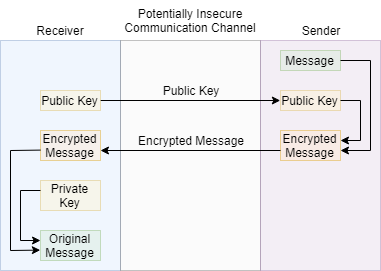
\includegraphics[scale=0.5]{rsa.png}
  \caption{RSA encryption}
\end{figure}

\paragraph{Key Generation} Keys are generated using two large primes, and this is what offers RSA
its high level of security once encrypted. The exact procedure is as follows:

\begin{enumerate}
\item Choose two distinct primes $p$ and $q$, at random. These are kept secret.
\item Compute $n = pq$. $n$ is used as the modulus, and its length expressed in bits is defined as
  the ``key length''. $n$ is part of the public key tuple.
\item Compute $\lambda (n)$, where $\lambda$ is Carmichael's totient function. Since $n=pq$,
  $$\lambda (n)  = \mathrm{LCM}(p-1, q-1)$$ $\lambda (n)$ is kept secret.
\item Choose integer $e$ such that $e$ and $\lambda (n)$ are coprimes. $e$ is usually set to
  $2^{16}+1 = 65537$, since it has a low Hamming weight (its binary representation has a lot of
  zeros). $e$ is called the public exponent.
\item Find $d$ by solving $$d\cdot e \equiv 1 \pmod{\lambda(n)}$$ that is, taking the modular multiplicative
  inverse of $e \pmod{\lambda(n)}$. $d$ is the private key and is kept secret.
\end{enumerate}

We hence have the public key tuple $(n, e)$ and the private key $d$. The above operations are
usually carried out using various optimized algorithms, which will be discussed while implementing
the Python code.

\subsubsection{RSA Proof and Example}
\paragraph{Fermat's Little Theorem}
Fermat's Little Theorem states that $a^{p-1} \equiv 1 \pmod{p}$ for any integer $a$ and prime $p$
not dividing $a$.

\paragraph{RSA Proof}
We are to show, $$(m^e)^d \equiv m \pmod{pq} \forall m$$ where $p$ and $q$ are distinct primes, and
$e$ and $d$ are positive integers satisfying $$ed \equiv 1 \pmod{\lambda (pq)}$$

Since $\lambda (n)  = \mathrm{LCM}(p-1, q-1)$, by construction, divisible by both $p-1$ and $q-1$:
$$ed - 1 = h(p-1) = k(q-1)$$ for some natural numbers $h$ and $k$.

From the Chinese Remainder Theorem,
\begin{displayquote}
  To check whether two numbers, like $m^{ed}$ and $m$, are congruent mod $pq$, it suffices (and in fact is equivalent) to check that they are congruent mod $p$ and mod $q$ separately.
\end{displayquote}

To show $m^{ed} \equiv m \pmod{p}$, we consider two cases:
\begin{enumerate}
  \item If $m \equiv 0 \pmod{p}$, $m$ is a multiple of $p$ (multiplicative cyclic group). Thus,
    $m^{ed}$ is a multiple of $p$. Thus, $m^{ed} \equiv 0 \equiv m \pmod{p}$.
  \item If $m \not\equiv 0 \pmod{p}$, $$m^{ed} = m^{ed-1}m = m^{h(p-1)}m \equiv 1^hm \equiv m
    \pmod{p}$$ where $m^{h(p-1)} \equiv 1^hm \pmod{p}$ by Fermat's Little Theorem.
\end{enumerate}

We proceed similarly for $q$, which completes the proof.

\paragraph{RSA Example}
The following is a simple proof of concept of RSA.
\begin{enumerate}
\item Let $p=11$, $q=3$.
\item $n=11 \times 3 = 33$
\item $\phi = (p-1)(q-1) = 20$. Note that we're not taking the LCM. \footnote{We are using Euler's
    rather than Carmichael's totient function. Any $d$ satisfying the former satisfies the latter,
    however, sometimes, Euler's yields a $d$ larger than required. In this case, the distinction is
    irrelevant. This doesn't matter for implements that use the Chinese Remainder Theorem, as $d$ is
    not used directly.}
\item Choose $e=3$.
\item Find $d$ such that $ed \equiv 1 \pmod{\phi}$. By trial and error, $d = 7$.
\item Hence, the public key is $(33, 3)$ and the private key is 7.
\item Let us encrypt $m=7$. $$c \equiv m^e \equiv 7^3 \equiv 343 \pmod{33} = 13$$ The ciphertext is
  hence 13.
\item Now, decrypting, $$m \equiv c^d \equiv 13^7 \pmod{33} = 7$$ We hence retrieve the original message.
\end{enumerate}


\cleardoublepage

\section{Python Implementation}
We now focus on building a complete RSA system in Python (3.6) that is capable of generating keys,
maintaining a database of users and their public/private keys, and encrypting and decrypting ASCII
text files of arbitrary length in reasonable time.

Wherever further mathematics is required for implementing a certain primitive or algorithm, it is
discussed prior its implementation in code.

\subsection{Installation}
The source code for this project is available on GitHub. You should either download it from
\url{https://github.com/nebhrajani-a/rsa-py} or clone it into a new directory.
\begin{verbatim}
$ git clone https://github.com/nebhrajani-a/rsa-py ./rsa-py
\end{verbatim}

\subsubsection{Dependencies}
The major non-standard dependancy is \texttt{progress}, which draws the progress bars during
encryptions and decryptions.
\begin{verbatim}
$ pip install progress
\end{verbatim}

Other (standard) dependancies are Python 3 (note that this program will \textbf{not} run on Python 2), math
(for the ceiling function), Secrets (secure random number generation), getpass (secure password
entry) and Pandas (database management).

\subsubsection{Compatibility}
This program is written to be platform independent, using Python implementations everywhere rather
than (possibly simpler) alternatives like command line calls. It's been tested on a machine running
Linux Mint 19.3 (XFCE 64-bit) and in two Microsoft Windows virtual machines (7 and 10), and behaves
as expected. If you think you are experiencing bugs, please write an email to \href{mailto:
aditya.v.nebhrajani@gmail.com}{aditya.v.nebhrajani@gmail.com}.


\subsubsection{Executing}
To use the program, \texttt{cd} to \texttt{/src} and execute
\begin{verbatim}
$ python main.py
\end{verbatim}


\textbf{Note:} If you use Windows, Python may be aliased to \texttt{py} instead. Make sure \texttt{python} runs Python 3 and not Python 2. On some Linux systems
Python 3 needs to be called using \texttt{python3}.


\subsection{Key Generation}
To generate keys, we must have: a large prime generator for $p$ and $q$, and math functions for
taking the LCM and modular multiplicative inverse of two numbers.

\subsubsection{Large Prime Generation}
Large prime generation is a mathematics problem as there is no evident pattern to finding primes.
$\pi(n)$ is the prime counting function for primes $\leq n$. According to the prime number
theorem\footnote{Which describes the asymptotic distribution of primes in the natural numbers. In fact, it is more explicitly stated as $\lim_{x\to\infty} \frac{\pi(x)}{x/ \ln{x}} = 1$.}
$$\pi(n) \sim \frac{n}{\ln{n}}$$

or the probability of a random $n$ being prime is $1/ \ln{n}$. For instance, the probability of a
random 2048 bit number being prime is $1/ \ln{2^{2048}} \approx 1/1419$.

\paragraph{Immediate Improvements} We can improve the previously calculated probability by noting
that no prime other than two is a multiple of two, meaning we have to check only half of the
otherwise required 1419 numbers, so $\sim 710$ numbers must be checked.

Now, to check if a number is prime, we need to divide it by every divisor $d$ such that $1 < d < n$.
There's another improvement here: we only have to check till $\sqrt{n}$ since if $n$ is composite and
equal to $pq$, either $p \leq \sqrt{n}$ or $q \leq \sqrt{n}$.

Or, in Python:
\begin{longlisting}
\begin{minted}{python}
def prime_generator(n):
    if n % 2 == 0:
        return False
    for i in range(3, sqrt(n), 2):
        if n % d == 0:
            return False
    return True
\end{minted}
\caption{Basic Prime Number Generator}
\end{longlisting}
This function certainly works, but has a time complexity $\mathcal{O}(\sqrt{n})$. This will need to
be faster for generating primes as large as 2048 bits. We hence turn to the probability based
Miller-Rabin primality test.

\paragraph{Non-Trivial Square Roots} We first define trivial and non-trivial square roots. The
trivial square roots of 1 $\mod{p}$ are 1 and $-1$, as they always return 1 on being squared modulo $p$, where
$p$ is a prime satisfying $p>2$.

We define a non-trivial square root of 1 $\mod{p}$ as any root other than 1 and $-1$. We prove now
that if such a root exists, $p$ cannot be prime (a special case of the result that, in a field, a
polynomial has as many zeros as its degree).

$$x^2 \equiv 1 \pmod{p}$$ $$(x-1)(x+1) \equiv 0 \pmod{p}$$

Which means $x \equiv 1$ or $-1 \pmod{p}$.

For example, consider $3^2 = 9 \equiv 1 \pmod{8}$, meaning 3 is a non-trivial square root of 1
$\mod{8}$. Clearly, 8 is composite.

\paragraph{Miller-Rabin Primality Test}
The Miller-Rabin test relies on finding nontrivial square roots of 1 $\mod{n}$.

Let $n$ be a prime and $n>2$. $n-1$ must be even, and we write it as $2^s\times d$, where $s$ and
$d$ are positive integers and $d$ is odd. For each $a$ in $(Z/nZ)\times$ (in range $[2, n-2]$),
either $$a^d \equiv 1 \pmod{n}$$ or $$a^{2^r\cdot d} \equiv -1 \pmod{n}$$ for some $0 \leq r \leq
s-1$. To prove the claim, check that by Fermat's Little Theorem, $a^{n-1} \equiv 1 \pmod{n}$. Hence,
if we repeatedly take the square roots of $a^{n-1}$, we will get either 1 or $-1$.

The Miller-Rabin test is the contrapositive of the above, that if we can find an $a$ such that both
of the above hold false, $n$ must be composite. $a$ is called a witness to the fact that $n$ is
non-prime. If some $a$ does not satisfy the negation of both the above, $a$ is called a strong liar,
and $n$ is a strong \emph{probable} prime for base $a$ (that is, it might yet be composite and still
hold the contrapositive).

Every odd composite number $n$ has many witnesses $a$, however, if we're unlucky, $a$ will be a strong
liar for $n$ and we'll categorize it as prime. There's no known way of generating an $a$ which isn't
a liar. We instead make the test probability based: we choose a random non-zero $a$ and test it.
Since it might be a strong liar, we repeat the test for a different value of $a$. The greater the
number of iterations we check, the higher is the probability of generating a prime $n$.

The time complexity of the Miller-Rabin test is $\mathcal{O} (k \log^3{n})$, which means it is a
polynomial time algorithm, a vast improvement over the simple method discussed earlier.

\paragraph{Final Implementation} We first generate a random number $n$ using Python's
\texttt{secrets} module. \footnote{The \texttt{random} module is not suitable for cryptographic
applications. Secrets instead calls the system's most secure source of randomness, such as /dev/random on
Linux.} We first implement a low level checker: we divide the randomly generated $n$ by every
element in a static list of the first 2000 primes. This eliminates obvious composite numbers early
on, speeding up our work. Also, this prevents some strong liars in Miller-Rabin. This is implemented
as follows:

\begin{longlisting}
\begin{minted}{python}
import first_primes as fp
import secrets

def gen_random(l):
    '''Generate a random number l bits long.'''
    randgenerator = secrets.SystemRandom()
    return randgenerator.randrange(2**(l-1)+1, 2**l - 1)
\end{minted}
\caption{$l$-bit Random Generator}
\end{longlisting}
Note that the random number generated is in the range $[2^{l-1}+1, 2^l-1]$ to ensure the correct
bit-length and to ensure that no extra even numbers are checked. Also note that
\texttt{first\_primes} is just a file with one list declaration. Files can be imported as modules in
Python 3 without an \texttt{\_\_init.py\_\_} file.

\begin{longlisting}
\begin{minted}{python}
def low_level_checker(l):
    '''Check that the random number isn't divisible by the first few primes.'''
    while True:
        x = gen_random(l)
        for divisor in first_primes:
            if x % divisor == 0 and divisor**2 <= x:
                break
        else: return x
\end{minted}
\caption{Low Level Primality Test}
\end{longlisting}
$n$ is then divided by every number in the first 2000 primes which is less than $\sqrt{n}$. Miller Rabin is then implemented exactly as described mathematically:

\begin{longlisting}
\begin{minted}{python}
def miller_rabin_checker(mrc):
    '''Run 40 iterations of the Miller-Rabin Primality Test.'''
    randgenerator = secrets.SystemRandom()
    max_divisions_by_two = 0
    y = mrc-1
    while y % 2 == 0:
        y >>= 1
        max_divisions_by_two += 1
    assert(2**max_divisions_by_two * y == mrc-1)

    def trial_composite(round_tester):
        if pow(round_tester, y, mrc) == 1:
            return False
        for i in range(max_divisions_by_two):
            if pow(round_tester, 2**i * y, mrc) == mrc-1:
                return False
        return True
    number_of_rabin_trials = 40
    for i in range(number_of_rabin_trials):
        round_tester = randgenerator.randrange(2, mrc)
        if trial_composite(round_tester):
            return False
    return True
\end{minted}
\caption{Miller-Rabin Primality Test}
\end{longlisting}
Note that the third argument of Python's \texttt{pow()} function takes an optional argument for the modulus.

Now that there is an implementation for both a low level and a high level checker (Miller-Rabin),
the last requirement is a driver function to actually generate the prime.

\begin{longlisting}
\begin{minted}{python}
def driver(l):
    while True:
        prime_candidate = low_level_checker(l)
        if not miller_rabin_checker(prime_candidate):
            continue
        else:
            return prime_candidate
\end{minted}
\caption{Prime Generation Driver}
\end{longlisting}
This driver function keeps generating random numbers until a number passes both the low level
checker and 40 iterations of Miller-Rabin\footnote{40 iterations were chosen from the reasoning in
\url{https://stackoverflow.com/a/6330138}}, which means it has an acceptably high probability of
being prime.

\subsubsection{Mathematics Functions}
Now that there is a framework for generating the random primes $p$ and $q$, a framework for taking
the LCM (lowest common multiple) and the modular multiplicative inverse is required.

\paragraph{LCM} For any integers $a$ and $b$, $ab = \mathrm{LCM}(a,b) \times \mathrm{GCD}(a,b)$.
Calculating the GCD (greatest common divisor or highest common factor) of two numbers is a simple
recursive algorithm called the (Standard) Euclidean Algorithm. It involves a succession of Euclidean
divisions (division with remainder).

First, take the larger of $a$ and $b$, the two numbers whose GCD we are to find. Divide the larger
(say $a$), by the smaller (say $b$). Then, divide $b$ by the remainder of this division. Continue to
take successive remainders as divisors for the next step and divisors for the former as dividends
for the latter. Continue this process until a remainder of zero is obtained. The divisor for this
operation is the GCD. The proof is trivial and well-known, so we skip to the Python implementation.

\begin{longlisting}
\begin{minted}{python}
import sys
sys.setrecursionlimit(10**6)

def gcd(a,b):
    if a == 0:
        return b
    return gcd(b % a, a)
\end{minted}
\caption{Recursive GCD Using Euclidean Algorithm}
\end{longlisting}
Note that the system recursion limit is increased to $10^6$ to prevent Python's stack overflow
inhibitor from kicking in for large numbers. While an iterative GCD function could be used,
recursive functions are funner and simpler to write. In addition, Python uses enough system
resources that this increase is not too resource-intensive. We do note, however, that Python is not
a functional language and an iterative implementation is a better choice for real world
applications.

The LCM is now trivial to calculate by simple division:

\begin{longlisting}
\begin{minted}{python}
def lcm(a,b):
    return (a*b) // gcd(a,b)
\end{minted}
\caption{LCM Finder Using GCD}
\end{longlisting}
`Floor' division is used as opposed to `true' division to prevent integer to float conversion, which
results in rounding and loss of LSB information.

\paragraph{Modular Multiplicative Inverse}
The modular multiplicative inverse is calculated using the Extended Euclidean Algorithm, which is
similar to the Standard Euclidean Algorithm used for calculating the GCD, except that the we use two
sequences rather than one. In the Standard Euclidean Algorithm the first divisors are represented
by $r_0 = a$ and $r_1 = b$ with the sequence following through $r_{i+1}=r_{i-1}-q_i r_i$ till
$r_{k+1} = 0$ and $r_k$ is the GCD.

In the Extended Euclidean Algorithm, the two sequences start with three values each, the first being
$r_0 = a$, $s_0 = 1$, $t_0 = 0$ and the other $r_1= b$, $s_1=0$, $t_1 = 1$. The sequence is followed
through $r_{i+1}=r_{i-1}-q_i r_i$, $s_{i+1}=s_{i-1}-q_i s_i$, $t_{i+1}=t_{i-1}-q_i t_i$, until we
find $r_{k+1} = 0$ and $r_k$ as GCD.

However, $s_k$ and $t_k$ are the Bézout coefficients of $a$ and $b$\footnote{The proof for this
claim is not within the scope of this paper.}. Bézout's identity is defined as:\footnote{From
Wikipedia, \url{https://en.wikipedia.org/wiki/B\%C3\%A9zout\%27s_identity}}

\begin{displayquote}
Bézout's identity — Let $a$ and $b$ be integers with greatest common divisor $d$. Then, there exist
integers $x$ and $y$ such that $ax + by = d$. More generally, the integers of the form $ax + by$ are
exactly the multiples of $d$.
\end{displayquote}
The Bézout's coefficients can be used to efficiently calculate the modular inverse, thus:
$ax + by = \mathrm{GCD}(a, b) = 1$ or, $ax - 1 = (-y)b$ or, $$ax \equiv 1 \pmod{b}$$

which completes our task. This algorithm runs in $\mathcal{O}(\log{b^2})$ time. The Python
implementation of the above two algorithms is as follows:

\begin{longlisting}
\begin{minted}{python}
def eea(a, b):
    '''Extended Euclidean algorithm'''
    if a == 0:
        return (b, 0, 1)
    else:
        g, y, x = eea(b % a, a)
        return (g, x - (b // a) * y, y)
\end{minted}
\caption{Extended Euclidean Algorithm}
\end{longlisting}
which is very similar to the recursive GCD algorithm, albeit with different sequences.

\begin{longlisting}
\begin{minted}{python}
def modinv(a, m):
    '''Find modular multiplicative inverse using EEA'''
    g, x, y = eea(a, m)
    if g != 1:
        raise Exception('Modular inverse does not exist.')
    else:
        return x % m
\end{minted}
\caption{Modular Inverse Using Extended Euclidean Algorithm}
\end{longlisting}
which simply calls \texttt{eea()} and takes the modulus.

\subsubsection{Putting It Together}
We are now set to generate keys, having all the required functions to do so. This is done as
outlined in Section~\ref{section:rsamath}. The code is self-explanatory.

\begin{longlisting}
\begin{minted}{python}
import prime_generator as pg
import math_functions as mf

def gen_keys(bits):
    p = pg.driver(bits//2)
    q = pg.driver(bits//2)
    n = p*q
    lambda = mf.lcm((p-1), (q-1))
    e = 65537
    d = mf.modinv(e, lambda)
    return [p, q, n, e, d, bits]
\end{minted}
\caption{Key Generator}
\end{longlisting}
\texttt{gen\_keys()} takes an argument for the bit-length of the resulting public key $n$, and
returns a list of the prime factors of $n$, $n$, the public and private keys, and the bit-length of
the public key. This data will be added to the user database eventually.

\subsection{Primitive RSA Encryption and Decryption}

Now that the keys have been generated, encryption and decryption is merely an exponentiation in
modulo $n$ as described in Section~\ref{section:rsamath}. The functions can hence be written as:
\begin{longlisting}
\begin{minted}{python}
def enc(m, e, n):
    c = pow(m, e, n)
    return c
\end{minted}
\caption{RSA Encryption}
\end{longlisting}
and,

\begin{longlisting}
\begin{minted}{python}
def dec(c, d, n):
    m = pow(c, d, n)
    return m
\end{minted}
\caption{Primitive RSA Decryption}
\end{longlisting}
The current implementation can be improved by using the Chinese Remainder Algorithm to speed up the
decryption process.

\subsubsection{Chinese Remainder Algorithm for Fast Decryption}
The Chinese Remainder Algorithm is a generalisation of the method used to solve problems such as:
\begin{displayquote}
There are certain things whose number is unknown. If we count them by threes, we have two left over;
by fives, we have three left over; and by sevens, two are left over. How many things are there?
\end{displayquote}
We use the following optimisation to decrypt, based on the general Chinese Remainder Theorem. The
following values are precomputed and stored as part of the private key:
\begin{enumerate}
\item $p$ and $q$: the primes from generation.
\item $d_P = d \pmod{p-1}$
\item $d_Q = d \pmod{p-1}$
\item $q_{inv} = q^{-1} \pmod{p}$
\end{enumerate}

We then use these four values to calculate the $c^d \pmod{pq}$ thus:
\begin{enumerate}
\item $m_1 = c^{d_P} \pmod{p}$
\item $m_2 = c^{d_Q} \pmod{q}$
\item If $m_1 > m_2$: $$h = q_{inv}(m_1 - m_2) \pmod{p}$$
\item Else: $$h = q_{inv}[(m_1 + \left \lceil{\frac{q}{p}}\right \rceil p) - m_2] \pmod{p}$$
\item $m = m_2 + hq \pmod{pq}$
\end{enumerate}

This algorithm derives its efficiency from calculating two small modular exponentiations rather than
one large one. The Python implementation is as follows:
\begin{longlisting}
\begin{minted}{python}
from math import ceil
def cra(c, p, q, d_p, d_q, q_inv):
    '''Chinese Remainder Algorithm'''
    m_1 = pow(c, d_p, p)
    m_2 = pow(c, d_q, q)
    if m_1 >= m_2:
        h = q_inv*(m_1-m_2) % p
    else:
        h = q_inv*((m_1 + (ceil(q/p))*p) - m_2) % p
    return pow((m_2 + h*q), 1, p*q)
\end{minted}
\caption{Chinese Remainder Algorithm for Fast Decryption}
\end{longlisting}
The decryption function then changes to:
\begin{longlisting}
\begin{minted}{python}
def dec(c, p, q, d_p, d_q, q_inv):
    m = mf.cra(c, p, q, d_p, d_q, q_inv)
    return m
\end{minted}
\caption{Decryption Using CRA}
\end{longlisting}

\subsection{ASCII to Integer via Octet Strings and Back}
Given all the previous algorithms and their implementations, we are ready to convert an integer message $m$
to ciphertext $c$ and back. However, one typically wishes to encrypt text, not an integer. We hence
define a few primitives to convert text to a long integer in a predictable and reversible way.

\subsubsection{PT2OS}
The first step is to convert individual letters to integers. Luckily for us, this is exactly how
letters are represented in computers, using ASCII octet strings. We hence write a Python function to
convert a string into a list of ASCII values (PlainText 2 (to) Octet String).

\begin{longlisting}
\begin{minted}{python}
def nochunk_PT2OS(text):
    return [ord(i) for i in text]
\end{minted}
\caption{Plain Text to Octet String}
\end{longlisting}

\subsubsection{OS2IP}
We must now convert the resulting octet string to an integer, which is done using the Octet String 2
(to) Integer Primitive. The PKCS\#1 standard defines OS2IP as follows~\cite{pkcs}:
\begin{displayquote}
\textbf{Input:} $X$, octet string to be converted

\textbf{Output:} $x$ corresponding nonnegative integer

\textbf{Steps:}
\begin{enumerate}
\item Let $X_1$ $X_2 \hdots X_n$ be the octets of $X$ from first to last, and let $X_i$ have the integer
  value $x_{l-i}$ for $1 \leq i \leq l$.
\item Let $x = x_{l-1} 256^{l-1} + x_{l-2} 256^{l-2} + . . . + x_1 256 + x_0$.
\item Output $x$.
\end{enumerate}
\end{displayquote}
The Python implementation is trivial:
\begin{longlisting}
\begin{minted}{python}
def OS2IP(X):
    l = len(X)
    i = 1
    sum_ = 0
    for X_i in X:
        sum_ = X_i*(256**(l-i)) + sum_
        i += 1
    return sum_
\end{minted}
\caption{OS2IP}
\end{longlisting}
Note that this is effectively a conversion to base 256. This integer will then be encrypted.

\subsubsection{I2OSP}
After decryption, we receive the base-256 integer again, and we must now restore it to an octet string. Or,
as the standard states (Integer 2 (to) Octet String Primitive):

\begin{displayquote}
\textbf{Input:}
$x$,        nonnegative integer to be converted
$l$,     intended length of the resulting octet string

\textbf{Output:}
$X$,        corresponding octet string of length $l$

\textbf{Error: }``Integer too large''

\textbf{Steps:}

1. If $x \geq 256^{l}$, output ``integer too large'' and stop.

2. Write the integer $x$ in its unique l-digit representation in
   base 256:

      $$x = x_{l-1} 256^{l-1} + x_{l-2} 256^{l-2} + \hdots
      + x_1 256 + x_0$$

   where $0 \leq x_i < 256$ (note that one or more leading digits will be
   zero if $x$ is less than $256^{l-1}$).

3. Let the octet $X_i$ have the integer value $x_{l-i}$ for $1 \leq i \leq l$.  Output the octet string
      $X = X_1 X_2 \hdots X_l$.
\end{displayquote}

The Python implementation of this is again simple, we merely divide $x$ and collect successive
remainders, recreating the octet string list.

\begin{longlisting}
\begin{minted}{python}
def I2OSP(x, l):
    if x >= 256**l:
        raise ValueError("Int too large.")
    i = 0
    X = []
    while i != (l-1):
        r = x % 256
        X.append(r)
        x = x // 256
        i += 1
    X.append(x)
    return X[::-1]
\end{minted}
\caption{I2OSP}
\end{longlisting}

\subsubsection{OS2PT}
We now are left with converting the octet string back to plaintext (Octet String 2 (to) PlainText),
which is another trivial operation in Python:
\begin{longlisting}
\begin{minted}{python}
def OS2PT(stream):
    return ''.join(chr(i) for i in stream)
\end{minted}
\caption{Octet String to Plain Text}
\end{longlisting}

\subsubsection{Putting It Together}
The order in which we apply the primitives is hence:

\begin{enumerate}
\item PT2OS
\item OS2IP
\item RSA Encrypt
\item RSA Decrypt (CRA)
\item I2OSP
\item OS2PT
\end{enumerate}

\subsection{File Chunking}

We can hence encrypt any plaintext whose integral value is less than the number of bits of
$n$.\footnote{To do this, select the \texttt{string} option when running the main program.} However,
very often, the requirement is to encrypt strings of far greater length called `files'. To encrypt a
file of arbitrary length, it must be split or `chunked' into multiple parts, each individually
encrypted, each individually decrypted, then woven back together.

To fulfill such a requirement, we first note that the file must be broken into equally sized chunks.
However, a file may not necessarily be perfectly divisible into chunks, that is, there will be a
remainder block which has insufficient bits. Hence, we pad the last block with a newline and ASCII
nulls, which will be removed later. This prevents corruption of the last block. To do so, we rewrite
PT2OS in the following way:
\begin{longlisting}
\begin{minted}{python}
def PT2OS(text, l):
    ret = [ord(i) for i in text]
    l_2 = len(ret)
    if l_2 < l:
        newline = [10]
        spaces = [0] * (l - l_2 -1)
        ret.extend(newline)
        ret.extend(spaces)
    return ret
\end{minted}
\caption{Chunking PT2OS}
\end{longlisting}
Note that 10 is an ASCII newline, which will be later removed. Now that the file is `chunkable', we
write a generator function which returns chunks of a specified size that we can later operate on.
\begin{longlisting}
\begin{minted}{python}
def read_in_chunks(file_object, chunk_size):
    '''Lazy function (generator) to read a file piece by piece.'''
    while True:
        data = file_object.read(chunk_size)
        if not data:
            break
        yield data
\end{minted}
\caption{Read File in Chunks Generator}
\end{longlisting}
And now, all that's left to do is remove the nulls from the last chunk after
decryption.\footnote{While the Pythonic way to write this function would be using texttt{with
open(filename):}, we use \texttt{f.open()} and \texttt{f.close()} for the sake of explicitness. They
are operationally the same.}
\begin{longlisting}
\begin{minted}{python}
def kill_nulls(filename):
    f = open(filename, 'r')
    lines = f.readlines()
    f.close()
    lines.pop()
    f = open(filename, 'w')
    for line in lines:
        f.write(line)
    f.close()
    f = open(filename, 'r')
    string = f.read()
    f.close()
    string = string[:-1]
    f = open(filename, 'w')
    f.write(string)
    f.close()
\end{minted}
\caption{Remove Extraneous Nulls}
\end{longlisting}
This function first reads the decrypted file line by line into a list, then deletes the last element
of the list, and writes the new list back to the file. It then reads the file into a string and
strips the newline from the end of the file, restoring the file to its pre-encryption state.

\subsection{User Data Pandas DataFrame}
This is the simpler part of our operation, we merely need to write functions to create a DataFrame
to act as a database file, and functions to add, remove, and search for data. This is the DataFrame
which maintains a list of users, their passwords, and their keys.

\paragraph{DataFrame Creation and Storage}
The DataFrame, once created, must be persistent across sessions. For this reason we save the
DataFrame as a Pickle (\texttt{.pkl} ) file.

\begin{longlisting}
\begin{minted}{python}
import pandas as pd

def save_table(usr_data):
    usr_data.to_pickle("usr_data.pkl")
\end{minted}
\caption{Pickle DataFrame}
\end{longlisting}
to create the DataFrame and,
\begin{longlisting}
\begin{minted}{python}
def read_table():
    return pd.read_pickle("usr_data.pkl")
\end{minted}
\caption{Read DataFrame Pickle}
\end{longlisting}
to read the created DataFrame.

Additionally, at level 0 indent, we must create the DataFrame if \texttt{usr\_data.pkl} doesn't
exist.
\begin{longlisting}
\begin{minted}{python}
from os import path
if not path.exists("usr_data.pkl"):
    usr_data = pd.DataFrame(columns = ['username', 'password', 'p', 'q', 'n', 'e', 'd_p', 'd_q', 'q_inv', 'bits'])
    usr_data.loc[0] = ['root', 0, 0, 0, 0, 0, 0, 0, 0, 0]
    save_table(usr_data)
\end{minted}
\caption{Create DataFrame}
\end{longlisting}
Note that the DataFrame stores the Chinese Remainder Algorithm parameters instead of the private key $d$.

\paragraph{Add And Remove Data}
\begin{longlisting}
\begin{minted}{python}
def add_data(data):
    usr_data = read_table()
    usr_data.loc[usr_data.index.max() + 1, :] = data
    save_table(usr_data)
\end{minted}
\caption{Add Data to DataFrame}
\end{longlisting}

\begin{longlisting}
\begin{minted}{python}
def drop_row(key):
    usr_data = read_table()
    index_ = get_index(key, 'user')
    usr_data.drop(index=index_, inplace = True)
    save_table(usr_data)
\end{minted}
\caption{Remove Data from DataFrame}
\end{longlisting}

\paragraph{Search For Data}
\begin{longlisting}
\begin{minted}{python}
def search_column(column, value):
    usr_data = read_table()
    result = (usr_data[usr_data[column] == value])
    if result.empty:
        return False
    else:
        return True
\end{minted}
\caption{Search DataFrame}
\end{longlisting}

\paragraph{Getting Fields And Indexes}

\begin{longlisting}
\begin{minted}{python}
def get_field(key, column):
    usr_data = read_table()
    x = usr_data.username[usr_data.username.str.contains('|'.join(key.split(' ')))]
    index = x.index[0]
    return usr_data.loc[index][column]
\end{minted}
\caption{Retrieve Field from DataFrame}
\end{longlisting}
Note that the actual integral value of the index is the first index of the Pandas Series datatype
that is assigned to $x$.

\begin{longlisting}
\begin{minted}{python}
def get_index(key, column):
    usr_data = read_table()
    x = usr_data.username[usr_data.username.str.contains('|'.join(key.split(' ')))]
    index = x.index[0]
    return index
\end{minted}
\caption{Retrieve Index from DataFrame}
\end{longlisting}

\subsection{Interaction Functions}
These are the functions that `talk' to the user and ask for inputs. They are fairly self
explanatory. While the ideal way to take inputs is a single command line which takes arguments,
these functions are written for the sake of providing a user-friendly front end to perhaps later
implement as a GUI.

\subsubsection{Users and Passwords}
First, prompt the user for account creation or signup:
\begin{longlisting}
\begin{minted}{python}
dimport usr_data as ud
import data_conversion_primitives as dcp
from getpass import getpass
import os.path

def login_or_signup():
    while True:
        try:
            state = int(input("[1] Create account\n[2] Sign in\n> "))
            if state not in (1, 2):
                print("ERR: Enter a valid choice.")
            else:
                return state
        except (TypeError, ValueError):
            print("ERR: Enter a valid choice.")
\end{minted}
\caption{Login/Signup Function}
\end{longlisting}
If the user wants to signup:

\begin{longlisting}
\begin{minted}{python}
def signup_core():
    while True:
        try:
            user = str(input("Enter a username:\n> "))
            if ud.search_column('username', user):
                print("Username taken, try another.")
            else:
                break
        except (TypeError, ValueError):
            print("Enter a valid username.")
    while True:
        try:
            passphrase_a = getpass(prompt = "Passphrase: ")
            passphrase_b = getpass(prompt = "Repeat passphrase: ")
            if passphrase_a == passphrase_b:
                passphrase_a = dcp.OS2IP(dcp.nochunk_PT2OS(passphrase_a))
                passphrase_a = pow(passphrase_a, 65537, 206013970136021274755909796996044923643)
                break
            else:
                print("Passphrases do not match. Try again.")
        except (ValueError, TypeError):
            print("Enter a valid passphrase.")
    return [user, passphrase_a]

def signup_pqned(data, pqned):
    data.extend(pqned)
    ud.add_data(data)
\end{minted}
\caption{Signup Function}
\end{longlisting}
The first function returns a list of the user's selected username and password, and the second
appends the key data to it after generation. This is then added to the DataFrame and pickled. Note
that passwords are \textbf{not} stored as plaintext, instead, they are actually RSA encrypted using
a static $(n,e)$. Note that this is done as an alternative to hashing the password.

If the user chooses to login, cross check data with the DataFrame and grant access.
\begin{longlisting}
\begin{minted}{python}
def login():
    while True:
        try:
            user = str(input("Enter your username:\n> "))
            if ud.search_column('username', user):
                break
            else:
                print("Username doesn't exist.")
        except (TypeError, ValueError):
            print("Enter a valid username.")
    while True:
        try:
            passphrase = getpass(prompt = "Passphrase: ")
            passphrase = dcp.OS2IP(dcp.nochunk_PT2OS(passphrase))
            passphrase = pow(passphrase, 65537, 206013970136021274755909796996044923643)
            if passphrase == ud.get_field(user, 'password'):
                break
            else:
                print("Incorrect passphrase. Try again.")
        except (TypeError, ValueError):
            print("Enter a valid passphrase.")
    return user
\end{minted}
\caption{Login Function}
\end{longlisting}
This concludes the login procedure.

\subsubsection{Get Functions}
To figure out what the user wants to do:
\begin{longlisting}
\begin{minted}[breaklines]{python}
def get_operation():
    while True:
        try:
            location = int(input("\n[1] File\n[2] String\n[3] Add path\n[4] Delete account\n[5] Exit\n> "))
            if location not in (1, 2, 3, 4, 5):
                print("ERR: Enter a valid choice.")
            else:
                return location
        except (TypeError, ValueError):
            print("ERR: Enter a valid choice.")
\end{minted}
\caption{Main Loop Operation Selector}
\end{longlisting}
If the user wants to operate on files, get the input file and the output file:

\begin{longlisting}
\begin{minted}{python}
def get_input_file():
    while True:
        filename = str(input("Input file?\n> "))
        try:
            with open(filename):
                return filename
        except FileNotFoundError:
            print("Incorrect file or path.")

def get_output_file():
    filename = str(input("Output file?\n> "))
    return filename
\end{minted}
\caption{File Management Functions}
\end{longlisting}
Choose whether to encrypt or decrypt:

\begin{longlisting}
\begin{minted}{python}
def encrpyt_or_decrypt():
    while True:
        try:
            state = int(input("[1] Encrypt file\n[2] Decrypt file\n> "))
            if state not in (1, 2):
                print("ERR: Enter a valid choice.")
            else:
                return state
        except (TypeError, ValueError):
            print("ERR: Enter a valid choice.")
\end{minted}
\caption{Encryption/Decryption Choice Function}
\end{longlisting}
Get encryption and decryption data:

\begin{longlisting}
\begin{minted}{python}
def get_encrypt_list(user):
    bits = ud.get_field(user, 'bits')
    e = ud.get_field(user, 'e')
    n = ud.get_field(user, 'n')
    return [bits, e, n]
def get_decrypt_list(user):
    bits = ud.get_field(user, 'bits')
    p = ud.get_field(user, 'p')
    q = ud.get_field(user, 'q')
    d_p = ud.get_field(user, 'd_p')
    d_q = ud.get_field(user, 'd_q')
    q_inv = ud.get_field(user, 'q_inv')
    return [bits, p, q, d_p, d_q, q_inv]
\end{minted}
\caption{Key Information Functions}
\end{longlisting}
When encrypting a file, select which user's public key to use:

\begin{longlisting}
\begin{minted}{python}
def get_reciever():
    while True:
        try:
            user = str(input("Enter recipient username:\n> "))
            if ud.search_column('username', user):
                break
            else:
                print("Username doesn't exist.")
        except (TypeError, ValueError):
            print("Enter a valid username.")
    return user
\end{minted}
\caption{Receiver Information Function}
\end{longlisting}
If the user wants to add a path to \texttt{sys.path}:
\begin{longlisting}
\begin{minted}{python}
def get_path():
    while True:
        path = str(input("Path?\n> "))
        if os.path.isdir(path):
            return path
        else:
            print("Not a valid path.")
\end{minted}
\caption{Path Validity Checker Function}
\end{longlisting}
Get the number of bits:
\begin{longlisting}
\begin{minted}{python}
def get_bits():
    print("Generating keys (one-time procedure).")
    while True:
        try:
            bits = int(input("Key length (bits)?\n> "))
            if bits >= 128 and mf.poweroftwocheck(bits):
                print("Key length okay...generating keys.")
                return bits
            else:
                print("ERR: Key length must be a power of two and greater than or equal to 128.")
        except (TypeError, ValueError):
            print("ERR: Enter a valid key length.")
\end{minted}
\caption{Interactive Bit-Length Finder}
\end{longlisting}
Since we need to check if the key input is a power of two, we write the following function:
\begin{longlisting}
\begin{minted}{python}
def poweroftwocheck(n):
    if (n == 0):
        return False
    while (n != 1):
        if (n % 2 != 0):
            return False
        n = n // 2
    return True
\end{minted}
\caption{Power of Two Checker}
\end{longlisting}

\subsubsection{Miscellaneous Functions}
If the user wants to delete their account:
\begin{longlisting}
\begin{minted}{python}
def del_user():
    user = login()
    ud.drop_row(user)
\end{minted}
\caption{User Deletion Interactive}
\end{longlisting}


\subsection{Putting It All Together}
Having created a library of functions, all that is left is assembling these correctly into a working
system. This is done as follows.

\subsubsection{Imported Modules}
\begin{longlisting}
\begin{minted}{python}
import rsa_primitive as rsa
import math_functions as mf
import data_conversion_primitives as dcp
import interaction_functions as intfunc
from progress.bar import IncrementalBar
import sys
\end{minted}
\caption{Main Module Imports}
\end{longlisting}
\texttt{progress} is used to draw the progress bars for encryption and decryption. \texttt{sys} will
be used to append paths.

\subsubsection{Signup And Login}
When the program is run, we call the login-related interaction functions.
\begin{longlisting}
\begin{minted}{python}
state = intfunc.login_or_signup()
if state == 1:
    data = intfunc.signup_core()
    bits = rsa.get_bits()
    pqned = rsa.gen_keys(bits)
    print("Keys successfully generated.")
    intfunc.signup_pqned(data, pqned)

user = intfunc.login()
\end{minted}
\caption{Main Signup and Login}
\end{longlisting}

The key generation process is done once for each user and stored in the database. After the signup
is completed, the user is asked to login to continue using the program. In case the user exists, go
directly to the login screen.

\subsubsection{Main Loop}
All the following code is wrapped in a forever loop. First, get the operation:
\begin{longlisting}
\begin{minted}{python}
operation = intfunc.get_operation()
\end{minted}
\caption{Main Operation Selection}
\end{longlisting}

\paragraph{File Encryption and Decryption}
Choose whether to encrypt or decrypt a file.
\begin{longlisting}
\begin{minted}{python}
if operation == 1:
    enc_or_dec = intfunc.encrpyt_or_decrypt()
\end{minted}
\caption{Main File Operation Selection}
\end{longlisting}
If encryption:
\begin{longlisting}
\begin{minted}{python}
if enc_or_dec == 1
    recpt = intfunc.get_reciever()
    input_file = intfunc.get_input_file()
    output_file = intfunc.get_output_file()
    enc_data = intfunc.get_encrypt_list(recpt)
    bits = enc_data[0]
    e = enc_data[1]
    n = enc_data[2]
    chunk_size = (bits//8) - 1
    open(output_file, 'w+').close()
    list_of_chunks = []
    fobj = open(input_file, 'r')
    l = sum(1 for _ in (dcp.read_in_chunks(fobj, chunk_size)))
    with open(input_file) as fin:
        print("All okay.")
        for data in
        IncrementalBar('Encrypting...', max=l).iter(dcp.read_in_chunks(fin, chunk_size)):
            data = dcp.PT2OS(data, chunk_size)
            data = dcp.OS2IP(data)
            data = rsa.enc(data, e, n)
            list_of_chunks.append(int(data))
    with open(output_file, 'a') as fout:
        print(list_of_chunks, end='', file=fout)
    print("Encrypted. Output written to", fout.name)
\end{minted}
\caption{Main Encryption Algorithm}
\end{longlisting}
The user first selects which file to encrypt (input) and which file to write to encrypted output to.
Note that these cannot be the same file. When encrypting a file, the public key of the recipient
must be retrieved from the database. The username of the recipient is requested, and the recipient's
public key retrieved from the database and read into variables $e$ and $n$. The output file is then
restored to an empty file state. The input file is read chunk by chunk, (the chunk size being
defined as one less than the byte length of $n$) and each chunk encrypted. The last chunk has nulls
added by PT2OS. Each chunk is written as an element of a list, which is written directly to the
file. The encrypted file is hence the output of printing a list to the output file.

Note that the \texttt{bar} variable creates the progress bar. For more details, see the
documentation of \texttt{progress}.

Else if decryption:

\begin{longlisting}
\begin{minted}{python}
else:
    input_file = intfunc.get_input_file()
    output_file = intfunc.get_output_file()
    dec_data = intfunc.get_decrypt_list(user)
    bits = dec_data[0]
    p = dec_data[1]
    q = dec_data[2]
    d_p = dec_data[3]
    d_q = dec_data[4]
    q_inv = dec_data[5]
    chunk_size = (bits//8) - 1
    open(output_file, 'w+').close()
    with open(input_file) as fin:
        list_of_chunks = fin.read()
    list_of_chunks = list_of_chunks.strip('][').split(', ')
    print("All okay.")
    f =  open(output_file, 'a')
    bar = IncrementalBar('Decrypting...', max=len(list_of_chunks))
    for data in list_of_chunks:
        data = rsa.dec(int(data), p, q, d_p, d_q, q_inv)
        data = dcp.I2OSP(data, chunk_size)
        data = dcp.OS2PT(data)
        print(data, end='', file=f)
        bar.next()
    f.close()
    dcp.kill_nulls(output_file)
    bar.finish()
    print("Decrypted. Output written to", f.name)
\end{minted}
\caption{Main Decryption Algorithm}
\end{longlisting}
When decrypting, first retrieve the private-key information of the user from the database. Ask for
the input and output files, and clear the output file. Then, read the input file into a list.
Decrypt each element in the list, add it to the output file, and close the output file. Then, kill
the nulls in the last chunk and exit.


\paragraph{String Encryption}
To encrypt a string using the user's own public key and decrypt it:
\begin{longlisting}
\begin{minted}{python}
elif operation == 2:
    enc_data = intfunc.get_encrypt_list(user)
    bits = enc_data[0]
    e = enc_data[1]
    n = enc_data[2]
    chunk_size = (bits//8) - 1
    dec_data = intfunc.get_decrypt_list(user)
    bits = dec_data[0]
    d = dec_data[1]
    p = dec_data[2]
    q = dec_data[3]

    m = str(input("Enter a string: "))
    m = dcp.PT2OS(m, chunk_size)
    m = dcp.OS2IP(m)

    c = rsa.enc(m, e, n)
    print("Encrypted string is:", m)
    m = rsa.dec(c, d, p, q)

    m = dcp.I2OSP(m, chunk_size)
    m = dcp.OS2PT(m)
    print("Decrypted string is:", m)
\end{minted}
\caption{Main String Encryption and Decryption}
\end{longlisting}

String encryption merely demonstrates basic encryption and decryption using the user's public and
private keys. The algorithm is self-explanatory.

\paragraph{Appending Path}
To append a path for file encryption:
\begin{longlisting}
\begin{minted}{python}
    elif operation == 3:
        path = intfunc.get_path()
        sys.path.append(path)
        print(sys.path[-1], "successfully appended to sys.path.")
\end{minted}
\caption{Main Append Path}
\end{longlisting}

The program can only access files to encrypt and decrypt which are in the \texttt{sys.path} list. To
add a path to that list, append it.

\paragraph{Account Deletion}
When the user wants to delete their account, confirm if they want to delete, ask for a login, then
delete.
\begin{longlisting}
\begin{minted}{python}
elif operation == 4:
    while True:
        try:
            sure = str(input("[ACCOUNT DELETION]: Proceed? Irreversible. (y or n): "))
            if sure not in ('y', 'n'):
                print("[ACCOUNT DELETION]: Please answer y or n.")
            else:
                if sure == "y":
                    intfunc.del_user()
                    print("All okay. Account successfully deleted.")
                    exit()
                else:
                    break
        except (TypeError, ValueError):
            print("[ACCOUNT DELETION]: Please answer y or n.")
\end{minted}
\caption{Main Account Deletion}
\end{longlisting}

\subsubsection{Exit}
To exit:
\begin{longlisting}
\begin{minted}{python}
    else:
        exit()
\end{minted}
\caption{Main Exit}
\end{longlisting}

\cleardoublepage


\section{Results}
The results in this section are sandbox tested on an Anaconda 3 install of Python on Microsoft
Windows 7 and 10, and on the standard Python 3 install on modern Linux systems.

\subsection{File Encryption Demonstration}

\begin{verbatim}
aditya@ganga:~$ python3 main.py
[1] Create account
[2] Sign in
>
\end{verbatim}
Create two accounts: one for the reciever and one for the transmitter. Also, test the passphrases should
match check.

\begin{verbatim}
[1] Create account
[2] Sign in
> 1
Enter a username:
> Rx
Passphrase:
Repeat passphrase:
Passphrases do not match. Try again.
Passphrase:
Repeat passphrase:
Generating keys (one-time procedure).
Key length (bits)?
> 2048
Key length okay...generating keys.
Keys successfully generated.
\end{verbatim}
Create transmitter account:

\begin{verbatim}
[1] Create account
[2] Sign in
> 1
Enter a username:
> Tx
Passphrase:
Repeat passphrase:
Generating keys (one-time procedure).
Key length (bits)?
> 2048
Key length okay...generating keys.
Keys successfully generated.
\end{verbatim}
Login as \texttt{Tx}, and encrypt a file using \texttt{Rx}'s public key. The standard test file
provided with the program is \texttt{file.txt}, a 3.7MB plaintext file that contains all Sherlock
Holmes stories, copyright-free. Note that 3.7MB of plaintext is on the larger side for plaintext files.

\begin{verbatim}
[1] Create account
[2] Sign in
> 2
Enter your username:
> Tx
Passphrase:

[1] File
[2] String
[3] Add path
[4] Delete account
[5] Exit
> 1
[1] Encrypt file
[2] Decrypt file
> 1
Enter recipient username:
> Rx
Input file?
> file.txt
Output file?
> encrypted_file.txt
All okay.
Encrypting... |--------------------------------| 15168/15168
Encrypted. Output written to encrypted_file.txt

[1] File
[2] String
[3] Add path
[4] Delete account
[5] Exit
> 5
aditya@ganga:~$
\end{verbatim}
Now, login as \texttt{Rx} and decrypt \texttt{encrypted\_file.txt}. Also, test if the input file
validity checker works. Note that decryption takes time on slower machines, so be patient.

\begin{verbatim}
[1] Create account
[2] Sign in
> 2
Enter your username:
> Rx
Passphrase:

[1] File
[2] String
[3] Add path
[4] Delete account
[5] Exit
> 1
[1] Encrypt file
[2] Decrypt file
> 2
Input file?
> not_a_real_file
Incorrect file or path.
Input file?
> encrypted_file.txt
Output file?
> decrypted_file.txt
All okay.
Decrypting... |--------------------------------| 15168/15168
Decrypted. Output written to decrypted_file.txt

[1] File
[2] String
[3] Add path
[4] Delete account
[5] Exit
> 5
aditya@ganga:~$
\end{verbatim}
Now, take a \texttt{diff} of the original \texttt{file.txt} and the decrypted \texttt{decrypted\_file.txt}.

\begin{verbatim}
aditya@ganga:~$ diff -s file.txt decrypted_file.txt
Files file.txt and decrypted_file.txt are identical
\end{verbatim}
Everything is working as expected, and there is no file corruption during transmission.


\subsection{String Encryption Demonstration}
Encrypt a string as user \texttt{Rx}:

\begin{verbatim}
[1] Create account
[2] Sign in
> 2
Enter your username:
> Rx
Passphrase:

[1] File
[2] String
[3] Add path
[4] Delete account
[5] Exit
> 2
Enter a string: Vi has two modes: beep repeatedly and break everything.
Encrypted string is: 426106800080092545292628332367505162029833888494867760168
244024768367189582946401783652132206259178410487838152923722727052684609932933
092094413439716313661863177446515975231556274621313114755645924171384324293295
384773762258024754518707293607592226811584111086257433522963820951094653987274
388815488587393422492138978777172905174711561625627364723028093682921917085995
341878452746452547249802532522505504037214403316278333042377377390429389015262
241861878095061253985069348804927368251210389257794265514066096280777415593309
365669989270930023422454615670637964006125830899578355259144369275599709533166
74813558784
Decrypted string is: Vi has two modes: beep repeatedly and break everything.
\end{verbatim}



\subsection{Account Deletion Demonstration}
Delete account \texttt{Tx}.
\begin{verbatim}
[1] Create account
[2] Sign in
> 2
Enter your username:
> Tx
Passphrase:

[1] File
[2] String
[3] Add path
[4] Delete account
[5] Exit
> 4
[ACCOUNT DELETION]: Proceed? Irreversible. (y or n): maybe
[ACCOUNT DELETION]: Please answer y or n.
[ACCOUNT DELETION]: Proceed? Irreversible. (y or n): y
Enter your username:
> Tx
Passphrase:
All okay. Account successfully deleted.
\end{verbatim}
Try to login with the deleted account:

\begin{verbatim}
[1] Create account
[2] Sign in
> 2
Enter your username:
> Tx
Username doesn't exist.
Enter your username:
>
\end{verbatim}
That concludes our demonstrations. To check the path addition and exit functions is trivial and
hence omitted.

\subsection{Encryption Time Test}
To test the time taken for encryption, we remove all user inputs and measure the time for purely the
encryption of \texttt{file.txt}. We run:

\begin{verbatim}
aditya@ganga:~$ for i in {1..10}; do time python3 enc_test.py; done
\end{verbatim}
The encryption tests take times between 10.2 and 10.8 seconds, as shown in the graph.

\begin{figure}[h]
  \centering
  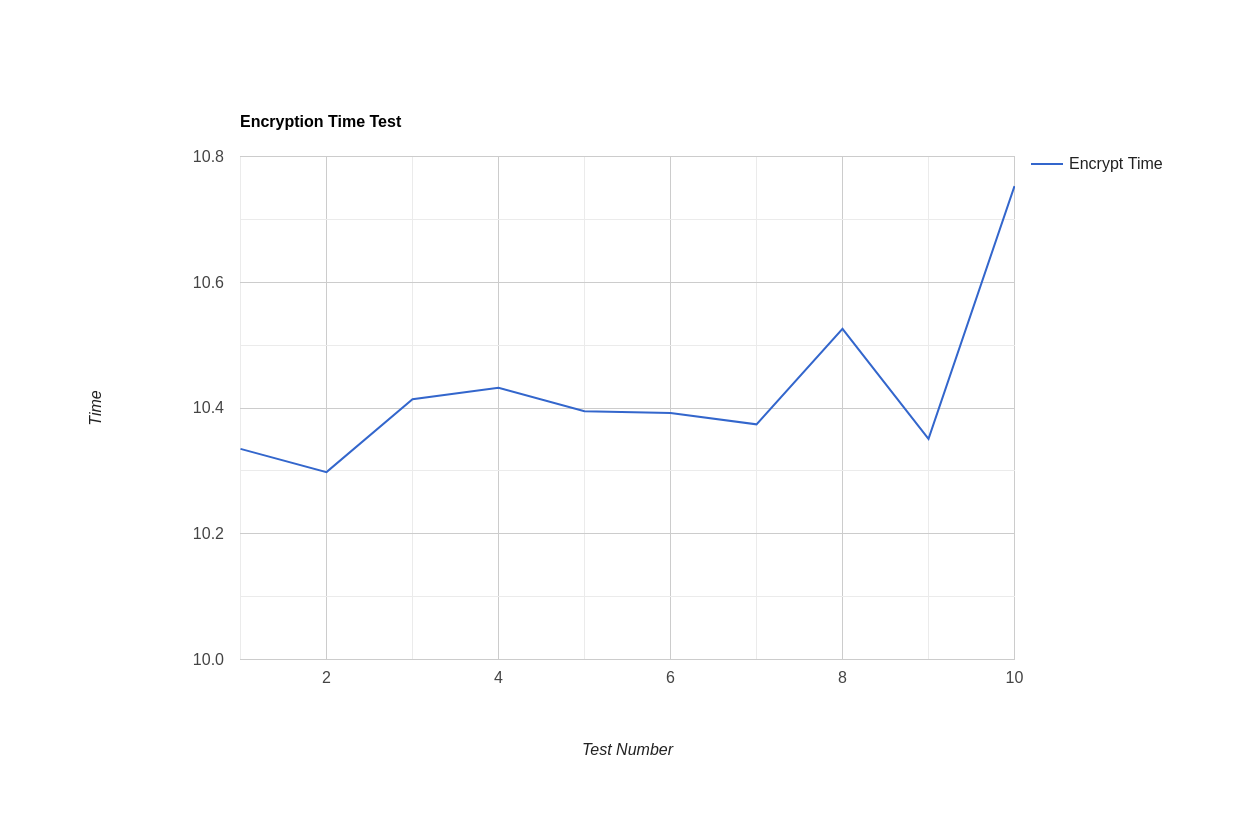
\includegraphics[scale=0.25]{eg.png}
  \caption{Encryption Time Graph}
\end{figure}

\subsection{Decryption Time Test}
Decryption takes longer than encryption, around 2 minutes 38 seconds on average. While this value is
a lot more than encryption, using the Chinese Remainder Algorithm speeds up the process greatly.
Using only Python's \texttt{pow()} function to decrypt took 8m19.523s.

\begin{verbatim}
aditya@ganga:~$ for i in {1..5}; do time python3 dec_test.py; done
\end{verbatim}


\begin{figure}[H]
  \centering
  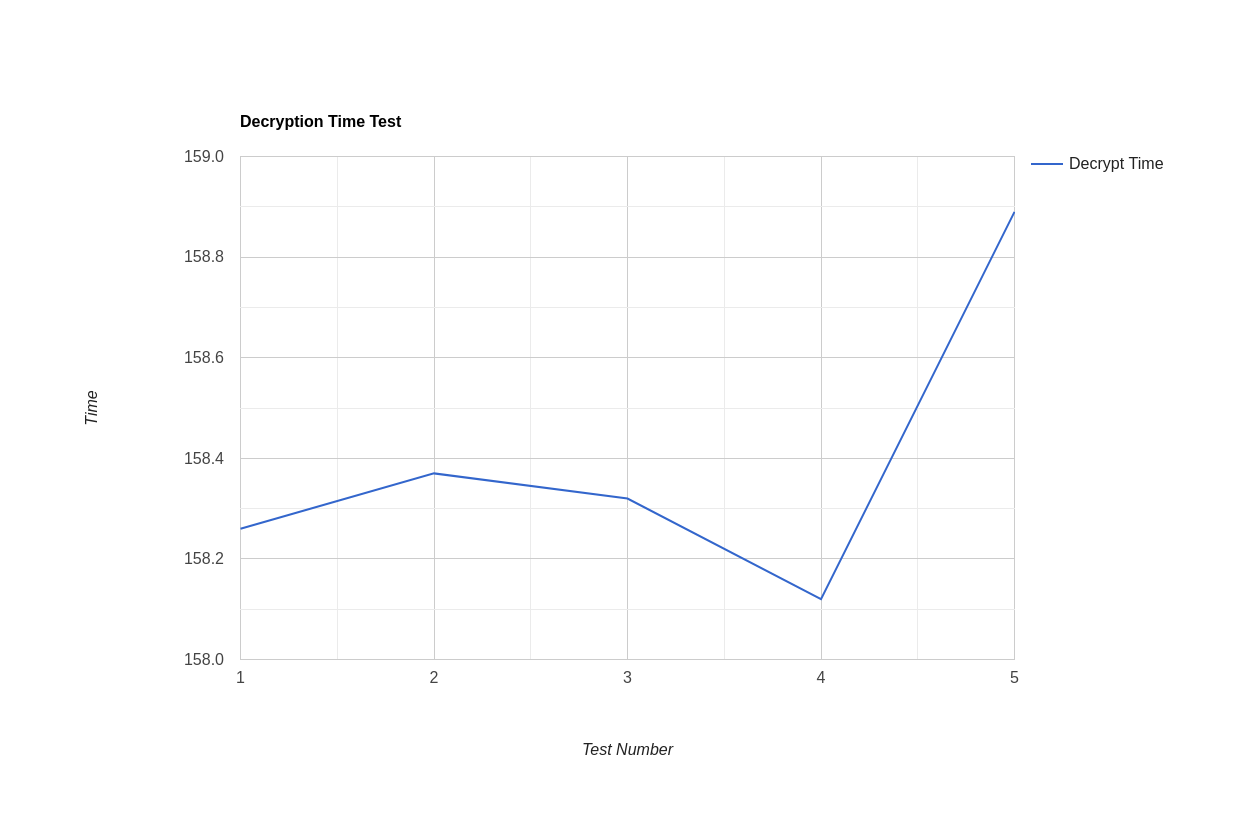
\includegraphics[scale=0.25]{dg.png}
  \caption{Decryption Time Graph}
\end{figure}
We have now completely tested the system created. In case of any discrepancies or improvements,
write an email to \href{mailto: aditya.v.nebhrajani@gmail.com}{aditya.v.nebhrajani@gmail.com}.



\cleardoublepage

\section{Author's Note}
\subsection{Public Key Cryptography Standard}
This tool implements the greater part of the PKCS (Public Key Cryptography Standard), with the
notable exception of OEAP padding. This part of the standard wasn't implemented due to time
constraints and other academic commitments. Padding is considered vital for short plaintexts, such
as those the string encryption implemented. However, for the length of plaintexts this tool
expects encryption for, padding is not so much a requirement as yet another compute-intensive task.
Given more time, I hope to eventually implement OAEP as well, complying with the standard
specified by PKCS.

\subsection{Tools}
% The only reason I was able to complete this project is standing on the shoulders of giants. In
% particular, the flexibility and power of the Linux system and GNU tools I used allowed me to
% complete this project orders of magnitude faster than any other platform. \\
% In particular, I would like to recommend GNU Emacs for code editing (admittedly with vi
% keybindings). Emacs with UNIX system tools such as \texttt{grep} are a development environment more
% powerful than any VS/Eclipse IDE. Emacs' endless customizability using LISP meant I could automate
% many parts of this project. In addition, I used VirtualBox for sandbox testing on Windows
% machines since I don't own any. VirtualBox brings virtualisation to anybody who may desire it, and
% behaves better than even Parallels desktop.\\
I am deeply indebted to the Python community and the creator of \texttt{progress}. While Python
is not functional and too high level for an application like this one, the fact that it could do it
this well, acting as both front end and back end (Pandas), makes it an excellent and powerful tool.
I hope to eventually implement a much better encryption/decryption tool in C to improve performance.
\footnote{Personally, I prefer statically typed, compiled languages with delimiters. In case the
source code of this project can be more Pythonic, please do let me know. There are many places where
I opted to write functions that could've been imported from various modules, since I believe the
only way to truly understand that code one writes is building it from scratch. Also, it increases
the translatablity of the code to languages with different libraries.} \\

The complete list of tools is:
\begin{multicols}{3}
\begin{itemize}
\item Foxconn Core i7 NanoPC.
\item Linux Mint 19.3 XFCE 64-bit.
\item GNU Emacs 25.2.2 (x86\_ 64-pc-linux-gnu, GTK+ Version 3.22.21),
  modified by Debian.
\item Python 3.6.9 from Debian repositories.
\item \LaTeX\ for documentation. pdf\TeX\ 3.14159265-2.6-1.40.18, from
  TeX Live 2017/Debian.
\item \LaTeX\ package \texttt{minted} for code highlighting.
\item Emacs \texttt{org-mode} 9.3.6, GNU ELPA.
\item GNU CLISP 2.49.60+ for some scripts.
\item VirtualBox 5.2.42 for sandbox.
\item Evince 2.4.4.
\end{itemize}
\end{multicols}


% Finally, the paper you are reading is formatted using \LaTeX, whose versatility and neat language
% are rivalled only by Emacs itself.

\subsection{This Paper}
This paper is written as a submission to the Central Board of Secondary Education (India) as an
Informatics Practices Investigatory Project for the year 2020-21. \\
It was noticed by the author of this paper that generally, investigatory projects, which are an
amazing opportunity to showcase computer science and mathematics-related talent, typically end up being
plagiarised programs from textbooks or the World Wide Web. In fact, the top ten results of an
Internet search for `CBSE IP Project', are all nearly identical ideas, with the same code and
errors. I hence perceive that on a general basis, students' participation is lacking in
investigatory projects.\\
This paper is an attempt to fully utilize the opportunity gracefully granted to me by CBSE and The
Orchid School, and to raise the bar for all students. It is my hope that this will inspire new and
fruitful work at the secondary level of education.\\
It has been my attempt to write this paper in the same way as a scholarly article insofar as I
could. If there are any errors or discrepancies, they remain my own.\\
I thank you for taking the time to go through this paper, and I hope you enjoyed reading it as much
as I enjoyed writing it.\\


\cleardoublepage


\section{Source Code by File}
This section directly highlights and prints from the \texttt{/src} directory. Other code snippets in
this document are static. If there is a change in source code, expect it to show up here first and
elsewhere in this document later.
\begin{verbatim}
ip_project/
|-- docs
|-- README.md
|-- src
\end{verbatim}

\subsection{prime\_generator.py}
\begin{longlisting}
\inputminted{python}{../src/prime_generator.py}
\caption{\textbf{File:} Prime Generator}
\end{longlisting}


\subsection{math\_functions.py}
\begin{longlisting}
\inputminted{python}{../src/math_functions.py}
\caption{\textbf{File:} Math Functions}
\end{longlisting}


\subsection{rsa\_primitive.py}
\begin{longlisting}
\inputminted{python}{../src/rsa_primitive.py}
\caption{\textbf{File:} RSA Primitive}
\end{longlisting}


\subsection{data\_conversion\_primitives.py}
\begin{longlisting}
\inputminted{python}{../src/data_conversion_primitives.py}
\caption{\textbf{File:} Data Conversion Primitives}
\end{longlisting}


\subsection{interaction\_functions.py}
\begin{longlisting}
\inputminted{python}{../src/interaction_functions.py}
\caption{\textbf{File:} Interaction Functions}
\end{longlisting}


\subsection{usr\_data.py}
\begin{longlisting}
\inputminted{python}{../src/usr_data.py}
\caption{\textbf{File:} User Data Management}
\end{longlisting}


\subsection{main.py}
\begin{longlisting}
\inputminted{python}{../src/main.py}
\caption{\textbf{File:} Main}
\end{longlisting}


\cleardoublepage


\printbibliography
\addcontentsline{toc}{section}{References}
\end{document}
